\documentclass[tikz,border=3pt]{standalone}
\usepackage[utf8]{inputenc}
\usepackage[T1]{fontenc}
\usepackage{lmodern}
\renewcommand{\familydefault}{\sfdefault}
\usepackage{sansmath}\sansmath
\usepackage{chemfig}
\usepackage{pgfplots}\pgfplotsset{compat=1.18,/pgf/number format/use comma,/pgf/number format/1000 sep={.}}
\usetikzlibrary{arrows.meta,calc,positioning,decorations.pathmorphing,patterns}
% paleta del sitio
\definecolor{nar}{HTML}{E8680C}\definecolor{narc}{HTML}{FFB35C}\definecolor{hielo}{HTML}{FFF3E8}
\definecolor{tinta}{HTML}{1D1D1F}\definecolor{gris}{HTML}{6E6E73}\definecolor{lila}{HTML}{7C5CF0}
\definecolor{azul}{HTML}{2F6FD6}\definecolor{menta}{HTML}{17A673}\definecolor{coral}{HTML}{E8342A}
\begin{document}
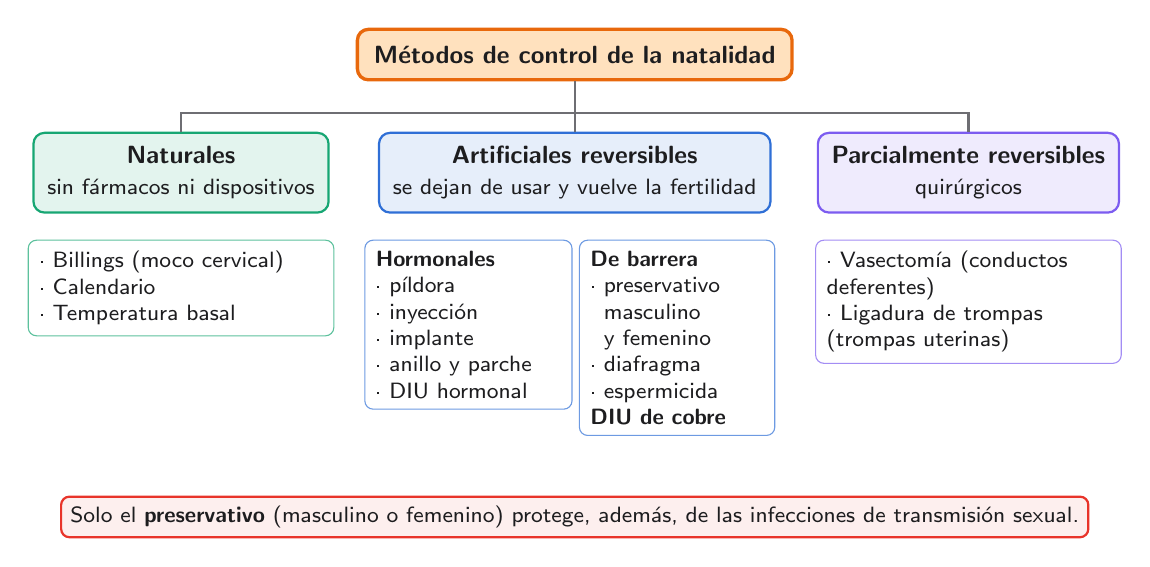
\begin{tikzpicture}[font=\small,
 raiz/.style={draw=nar,very thick,fill=narc!40,rounded corners=4pt,align=center,inner sep=6pt,text=tinta,font=\small\bfseries},
 cat/.style={draw=#1,thick,fill=#1!12,rounded corners=4pt,align=center,inner sep=5pt,text=tinta,minimum width=3.6cm},
 hoja/.style={draw=#1!70,fill=white,rounded corners=3pt,align=left,inner sep=4pt,text=tinta,font=\footnotesize,text width=3.4cm},
 l/.style={gris,thick}]
\node[raiz] (r) at (0,0) {Métodos de control de la natalidad};
\node[cat=menta] (n) at (-5.0,-1.5) {\textbf{Naturales}\\\footnotesize sin fármacos ni dispositivos};
\node[cat=azul] (a) at (0,-1.5) {\textbf{Artificiales reversibles}\\\footnotesize se dejan de usar y vuelve la fertilidad};
\node[cat=lila] (q) at (5.0,-1.5) {\textbf{Parcialmente reversibles}\\\footnotesize quirúrgicos};
\draw[l] (r.south) -- ++(0,-0.4) -| (n.north); \draw[l] (r.south) -- (a.north); \draw[l] (r.south) -- ++(0,-0.4) -| (q.north);
\node[hoja=menta,anchor=north,text width=3.6cm] at (-5.0,-2.35) {· Billings (moco cervical)\\· Calendario\\· Temperatura basal};
\node[hoja=azul,anchor=north,text width=2.35cm] (h) at (-1.35,-2.35) {\textbf{Hormonales}\\· píldora\\· inyección\\· implante\\· anillo y parche\\· DIU hormonal};
\node[hoja=azul,anchor=north,text width=2.2cm] (b) at (1.3,-2.35) {\textbf{De barrera}\\· preservativo\\\phantom{· }masculino\\\phantom{· }y femenino\\· diafragma\\· espermicida\\\textbf{DIU de cobre}};
\node[hoja=lila,anchor=north,text width=3.6cm] at (5.0,-2.35) {· Vasectomía (conductos deferentes)\\· Ligadura de trompas (trompas uterinas)};
\node[draw=coral,thick,rounded corners=3pt,fill=coral!8,text=tinta,font=\footnotesize,align=center,anchor=north] at (0,-5.6) {Solo el \textbf{preservativo} (masculino o femenino) protege, además, de las infecciones de transmisión sexual.};
\end{tikzpicture}
\end{document}
